\documentclass[a4paper, 10pt]{article}
\usepackage[utf8x]{inputenc}
\usepackage{graphicx}
\usepackage{geometry}
\usepackage{amsmath}
\usepackage{mathenv}
\usepackage{amssymb}
\usepackage{amsfonts}
\usepackage{mathrsfs}
\usepackage{textcomp}
\usepackage{subfigure}
\usepackage{graphics}
\usepackage{pstricks,pstricks-add,pst-math,pst-xkey}
\usepackage{multicol}
\geometry{hmargin = 2.5cm, vmargin = 1.5cm}

% OPENING
\title{SY19 - TP01\\Positionnement multidimensionnel}
\author{Alice Ngwembou - Antoine Hars}

\begin{document}

\maketitle

\section*{Introduction}
Au cours de ce tp, nous étudions les différentes types de techniques de positionnement\\multidimensionnel, dans un premier temps théoriquement,
puis dans un second temps sur différents types de données (\textit{mutations} et \textit{airport}) au moyen de fonctions de R.

\section*{Exercice 1 : Exercice théorique}
\subsection*{Première partie : ACP}
% QUESTION 1.1
\textbf{Question 1 :}\\
Afin de calculer les axes factoriels de l'ACP du nuage de points définis, nous centrons, dans un premier temps, la matrice donnée,
ce qui nous permet de prendre comme nouvele origine le centre de gravité dans l'espace des individus.\\
Nous calculons ensuite la matrice de covariance \textit{S} pour appliquer la fonction \textit{eigen()} sur cette dernière,
ce qui nous donne les résultats suivants :\\ \\
\begin{tabular}{|c|c|c|c|c|c|c|c|c|}
\hline
 & $\lambda1$ & $\lambda2$ & $\lambda3$ & $\lambda4$ & $\lambda5$ & $\lambda6$ & $\lambda7$ & $\lambda8$ \\
\hline
Valeurs propres & 24.26 & 0.006 & 3.85e-16 & 3.65e-17 & 1.52e-19 & -1.84e-19 & -7.17e-16 & -1.50e-15 \\
\hline
Inerties expliquées & 98.45\% & 100\% & 100\% & 100\% & 100\% & 100\% & 100\% & 100\% \\
\hline
\end{tabular}\\
\textit{Tableau des valeurs propres et obtenues sur le nuage de points définis.}\\ \\
D'après les valeurs obtenues, nous pouvons dire que seules les 2 premières valeurs de valeur propres sont intéressantes car les valeurs
suivantes sont excessivement proches de zéro (positives ou négatives) mais nous veillons à calculer les inerties expliqués en nous
basant sur la somme des valeurs absolues des valeurs propres.\\
Nous pouvons donc remarquer que les 2 premiers axes factoriels, donc le plan factoriel défini par ces 2 axes,
cumulent environ 100\% de l'information.\\ \\
% QUESTION 1.2
\textbf{Question 2 :}\\
La matrice de composantes principales nous permettent de représenter les 8 individus dans le premier plan factoriel :\\
\hspace*{0.5cm}
\begin{tabular}{c}
$C = X * M * U =
\begin{pmatrix}
-3.62 & 0.60 \\
2.47 & 0.29 \\
4.54 & -0.18 \\
-4.47 & 0.07 \\
-3.09 & -0.24 \\
3.69 & -0.71 \\
-3.52 & -0.51 \\
4.01 & 0.67
\end{pmatrix}$\\
\end{tabular}
\hspace*{1cm}
\begin{tabular}{c}
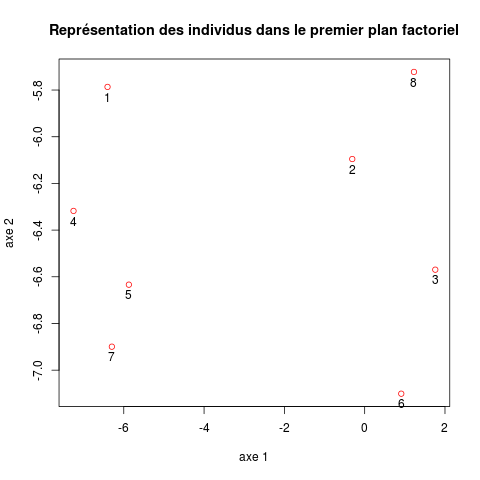
\includegraphics[height = 5cm, width = 5cm]{plots/biplot_exo1_princomp.png}\\
\end{tabular}\\
L'ACP applique un changement de base au jeu de données car on a cherché à obtenir une représentation fidèle du nuage de points en
le projetant sur un espace de plus faible dimension (dans notre cas, de dimension 2) sans perdre trop d'informations.
Les variables obtenues par la projection sont donc des combinaisons linéaires des variables du nuage initial.
\newpage
\noindent
% QUESTION 1.3
\textbf{Question 3 :}\\
$\varSigma^{k}_{\alpha=1} c_{\alpha}u_{\alpha}'$ pour \textit{k = 1} et \textit{k = 2} nous permet de retrouver notre matrice X de départ,
à savoir la matrice contenant le jeu de données : $X = \varSigma^{k}_{\alpha=1} c_{\alpha}u_{\alpha}'$.

\subsection*{Deuxième partie : MDS}
% QUESTION 2.1
\textbf{Question 1 :}\\
Le calcul de \textit{$D^{2}$} nous donne le tableau suivant (utilisation de la méthode R $dist(X, method = "euclidian")$):\\ \\
$D^{2}$ = 
\begin{tabular}{|ccccccc|}
37.25 & & & & & & \\
67.25 & 4.50 & & & & & \\
1.00 & 48.25 & 81.25 & & & & \\
1.00 & 31.25 & 58.25 & 2.00 & & & \\
55.25 & 2.50 & 1.00 & 67.25 & 46.25 & & \\
1.25 & 36.50 & 65.00 & 1.25 & 0.25 & 52.00 & \\
58.25 & 2.50 & 1.00 & 72.25 & 51.25 & 2.00 & 58.00 \\
\end{tabular}\\ \\
% QUESTION 2.2
\textbf{Question 2 :}\\
Pour calculer la matrice des produits scalaires \textit{W}, 2 méthodes sont possibles :

- En utilisant la matrice centrée des données de départ \textit{X} : \textit{W = X * $X^{t}$}

- En partant du tableau des distances euclidiennes \textit{$D^{2}$} : \textit{W = $-\frac{1}{2} * Q_{n} * D^{2} * Q_{n}$} avec $n = 8$\\ \\
% QUESTION 2.3
\textbf{Question 3 :}\\
Pour déterminer si $W$ ou $\frac{1}{n}W$ est semi-définie positive, nous devons observer si les valeurs propres de la matrice $\frac{1}{n}W$
sont positives :\\
Le calcul des valeurs propres nous donne le même résultat que celui trouvé à partir de la matrice de covariance $S$ dans la première partie.
Nous pouvons donc observer que nous avons 5 valeurs positives (dont 3 valeurs comprises entre $10^{-16}$ et $10^{-19}$) et
3 valeurs négatives (comprises entre $10^{-19}$ et $10^{-15}$), nous choisissons donc de les considérer comme nulles vu qu'elles sont minimes
(vu que les 2 premières valeurs propres regroupent environ 100\% de l'information).\\
Donc vu que nous disposons de valeurs positives et nulles, la matrice $W$ est semi-définie positive.\\ \\
% QUESTION 2.4
\textbf{Question 4 :}\\
La matrice diagonale des valeurs propres $L$ est obtenue par la formule suivante : $L = \lambda * I_{n}$, avec $\lambda$ correspondant
au vecteur colonne des valeurs propres de $\frac{1}{n}W$.\\
La matrice des vecteurs propres normés $V$ est obtenue via l'expression suivante : $V = \sqrt{n}\frac{1}{n}U$ avec $U$ la matrice des vecteurs
propres de $W$.\\ \\
% QUESTION 5
\textbf{Question 5 :}\\
Nous obtenons la représentation fournie par l'\textit{AFTD} avec l'expression des composantes principales\\suivantes : $C = V\sqrt{L}$.\\ \\
% QUESTION 6
\textbf{Question 6 :}\\
La représentation de $X$ et celle fournit par l'\textit{AFTD} nous donne les graphiques suivants :\\
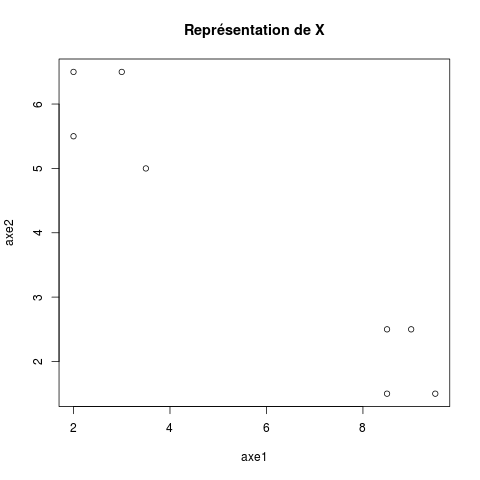
\includegraphics[height = 6cm, width = 6cm]{plots/plot_exo1.png}
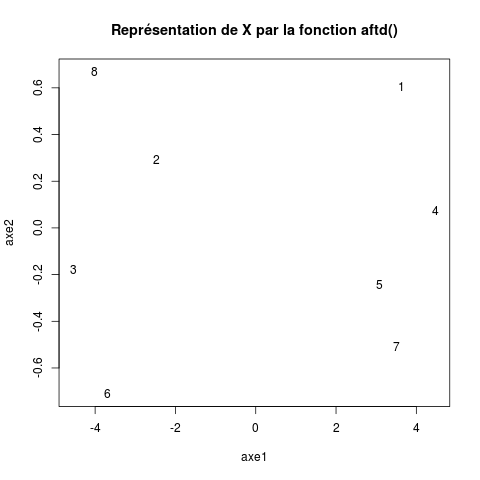
\includegraphics[height = 6cm, width = 6cm]{plots/plot_exo1_aftd.png}\\
Nous remarquons sur les 2 graphiques que nous avons 2 classes d'individus bien identifiés.
La représentation par l'\textit{AFTD} réduit les distances qu'il y a entre chaque point.
\newpage
\noindent
% QUESTION 7
\textbf{Question 7 :}\\
La fonction \textit{aftd()} créée est la suivante :
\begin{verbatim}
aftd <- function (d) {

  # Transformation de la matrice de distances en matrice
  dim_mat = as.matrix(d)
  d2 = dim_mat^2

  # Récupération de la première dimension de la matrice (nbre de lignes = nbre d'individus)
  dimension = diag(dim(dim_mat))[1]

  # Création de la matrice identité
  id = diag(dimension)

  # Création de la matrice unitaire
  un = matrix(rep(1, dimension^2), dimension)

  # Création de la matrice Q de centrage
  q = id - (1/dimension) * un

  # Calcul de la matrice w
  w = -(1/2) * q %*% d2 %*% q

  # Matrice associée aux vecteurs propres
  V = eigen(1 / dimension * w)$vectors[,1:dimension]
  V = sqrt(dimension) * V

  # Matrice associées aux valeurs propres
  L = diag(c(eigen(1 / dimension * w)$values[1:dimension]))

  # Calcul composante principale
  C = V %*% sqrt(L)

  # Calcul du pourcentage d'inertie pour les 7 premières valeurs propres
  quality = sum(diag(L)) / sum(eigen(1 / dimension * w) $values) * 100

  result <- new.env()
  result$quality <- quality
  result$C <- C
  return(result)
}

\end{verbatim}


\section*{Exercice 2 : Les données de mutations}
% QUESTION 1
\textbf{Question 1 :}\\
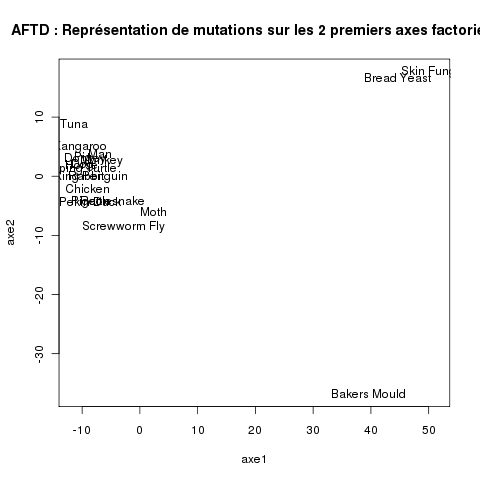
\includegraphics[height = 7cm, width = 7cm]{plots/plot_mutations_aftd.png}
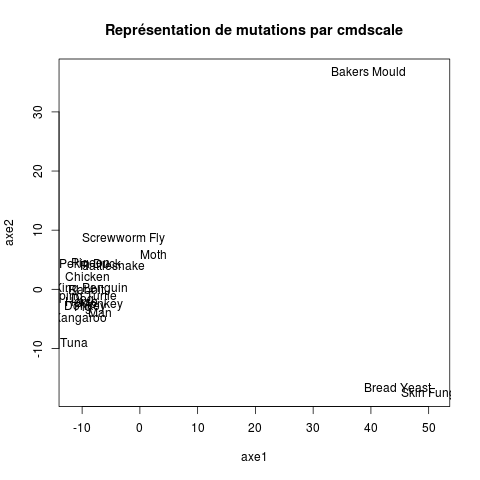
\includegraphics[height = 7cm, width = 7cm]{plots/plot_mutations_cmdscale.png}\\ \\
Les représentations de notre fonction \textit{aftd()} et de la fonction \textit{cmdscale()} sont similaires,
on peut\\observer 3 groupes d'espèces bien différenciés entre eux.\\ \\
% QUESTION 2
\textbf{Question 2 :}\\
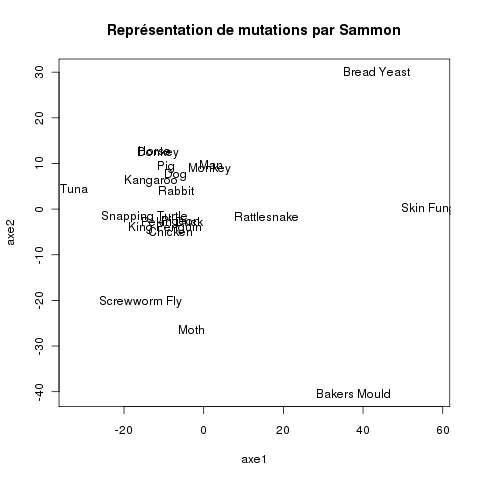
\includegraphics[height = 7cm, width = 7cm]{plots/plot_mutations_sammon.png}
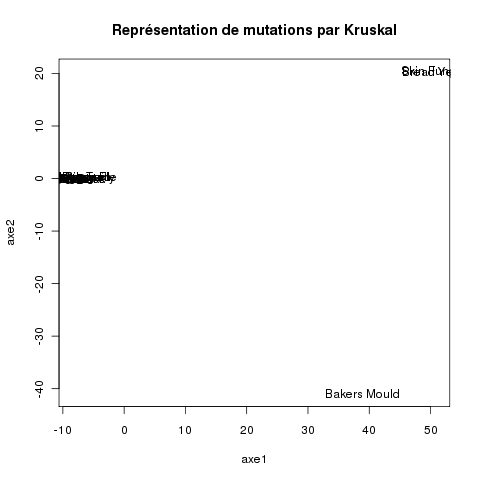
\includegraphics[height = 7cm, width = 7cm]{plots/plot_mutations_kruskal.png}\\ \\
La représentation de \textit{Kruskal} nous montre les 3 groupes présents sur les 2 représentations de l'\textit{AFTD} précédentes,
cependant, les individus de chaque groupe sont beaucoup plus concentrés sur un même point, les distances entre les individus sont minimes.\\
Concernant la méthode de \textit{Sammon}, nous pouvons observer au contraire que les individus sont plus\\dispersés par rapport aux autres
représentations. Nous n'avons pas 3 groupes d'individus bien définis. La projection par cette méthode ne tend pas à minimiser les distances
entre chaque individus du nuage de points initial.\\
L'\textit{AFTD} semble être une méthode pour donner une représentation intermédiaire entre les méthodes de \textit{Kruskal} et de
\textit{Sammon}.\\ \\
% QUESTION 3
\textbf{Question 3 :}\\
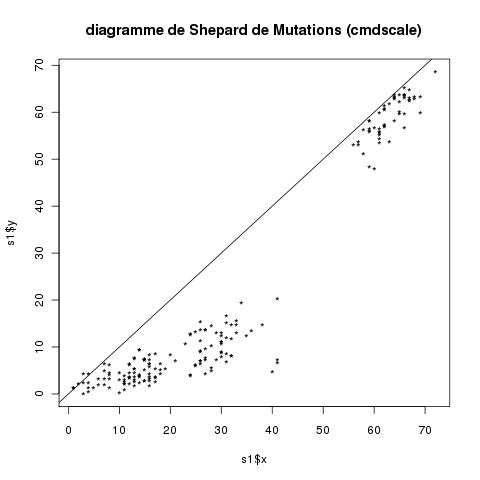
\includegraphics[height = 5cm, width = 5cm]{plots/plot_mutations_shepard_cmdscale.png}
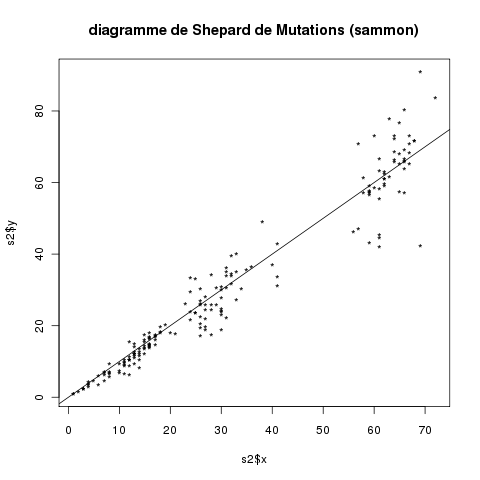
\includegraphics[height = 5cm, width = 5cm]{plots/plot_mutations_shepard_sammon.png}
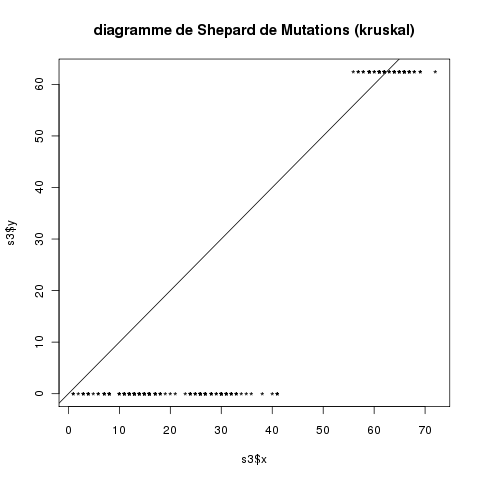
\includegraphics[height = 5cm, width = 5cm]{plots/plot_mutations_shepard_kruskal.png}\\ \\
Ces diagrammes de \textit{Shepard} nous permettent d'apprécier la qualité des projections de données par les différentes méthodes
(\textit{AFTD}, \textit{Sammon} et \textit{Kruskal}).
Pour la méthode de l'\textit{AFTD}, nous remarquons que la projection des individus et sous-estimée.
Pour la méthode de \textit{Sammon}, la projection des individus a tendance à suivre la diagonale, ce qui nous indique que la méthode de
\textit{Sammon} nous donne une projection de meilleure qualité par rapport à la précédente.\\
La qualité de représentation de la méthode de \textit{Kruskal} est la plus faible des 3.
Nous remarquons que \textit{Kruskal} minimise au maximum la distance entre les individus, ce qui nous donne une vue globale plus claire,
ce qui nous permet de dégager les groupes d'individus plus facilement alors que la méthode de \textit{Sammon} nous permet d'étudier
les distances entre chaque individus de manière plus fiable.
L'\textit{AFTD} nous permet une représentation intermédiaire.\\ \\

\section*{Exercice 3 : Les données de distances entre aéroports}
Dans cet exercice, nous travaillons sur les données contenues dans le fichier \textit{airport2.txt} qui représentent les distances de vol
entre des aéroports situés dans le monde. L'objectif de cet exercice est d'appliquer les différentes méthodes
de positionnement multidimensionnel à ces données et de comparer les résultats obtenus.\\ \\
L'exécution des méthodes de l'\textit{AFTD}, de \textit{Sammon} et de \textit{Kruskal} sur le tableau de distance des données
nous donne les graphiques suivants :\\
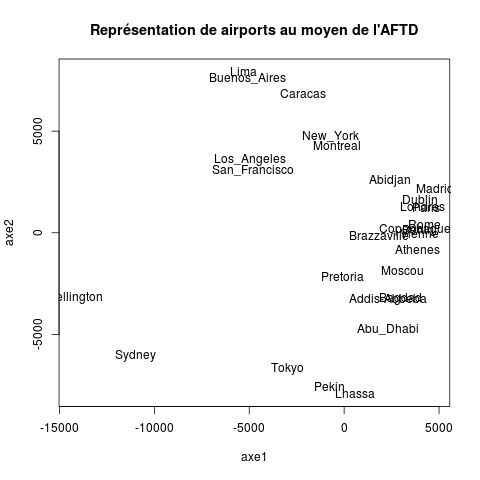
\includegraphics[height = 5cm, width = 5cm]{plots/plot_airports_cmdscale.png}
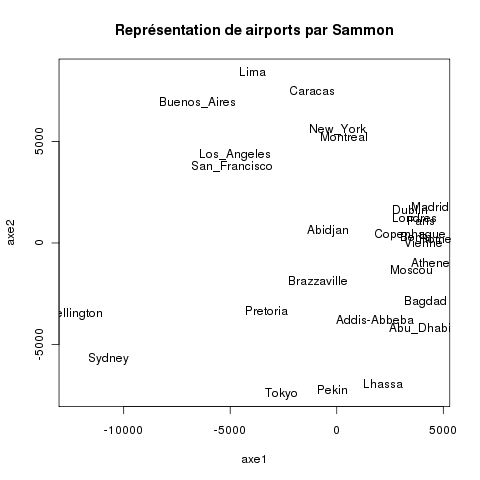
\includegraphics[height = 5cm, width = 5cm]{plots/plot_airports_sammon.png}
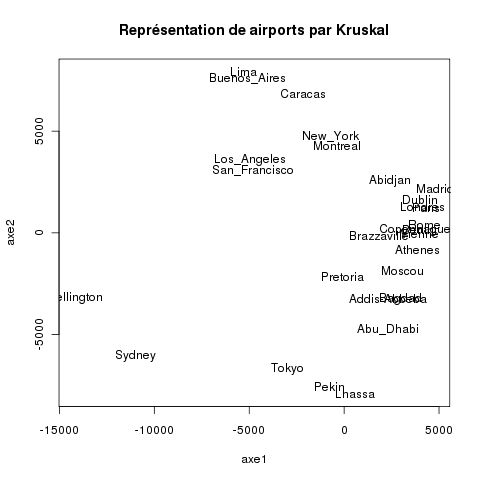
\includegraphics[height = 5cm, width = 5cm]{plots/plot_airports_kruskal.png}\\ \\
% QUESTION 1
\textbf{Question 1 :}\\
À travers la représentation de l'\textit{AFTD} (fonction \textit{cmdscale}), nous pouvons observer que les différents continents ressortent plus ou moins
entre eux.
Nous avons l'Amérique en haut du graphique, l'Europe au centre et les pays orientaux en bas du graphique.
Vu que les distances ont été calculées dans un référentiel en 3 dimensions, la représentation de ces distances dans un référentiel en 2 dimensions
altère le positionnement des aéroports entre eux mais l'ensemble reste cohérent.\\ \\
% QUESTION 2
\textbf{Question 2 :}\\
La représentation de \textit{Sammon} présente une répartition globale des éléments similaire à la représentation de l'\textit{AFTD}.
À l'intérieur de chaque groupe d'aéroports, nous notons cependant des différences\\sensibles (Tokyo, Pékin et Lhassa sont positionnées
différemment).
Quant à la représentation de \textit{Kruskal}, nous remarquons une disposition des aéroports similaire à la représentation de l'\textit{AFTD}.
La différence de représentation entre celle de \textit{Sammon} et celles de \textit{Kruskal} et de l'\textit{AFTD} provient vraisemblablement
du changement de dimension appliqué pour obtenir une représentation sur 2 axes de distances obtenues dans 3 dimensions.\\ \\
Pour comparer ces 3 représentations, nous observons les diagrammes de Shepard associés :\\
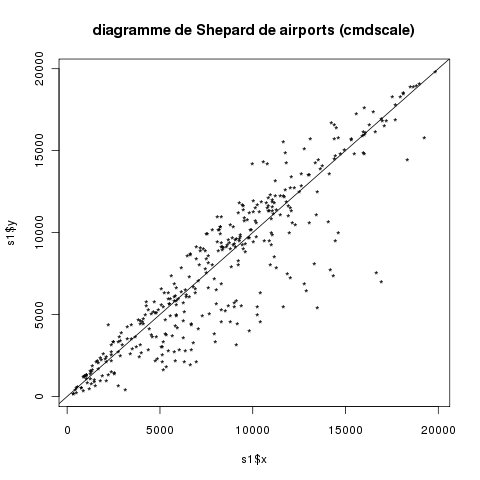
\includegraphics[height = 5cm, width = 5cm]{plots/plot_airports_shepard_cmdscale.png}
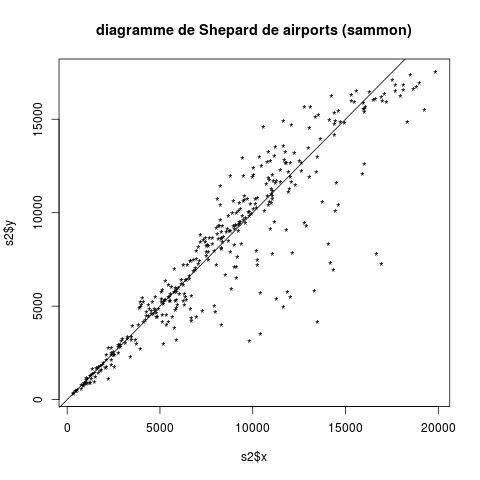
\includegraphics[height = 5cm, width = 5cm]{plots/plot_airports_shepard_sammon.png}
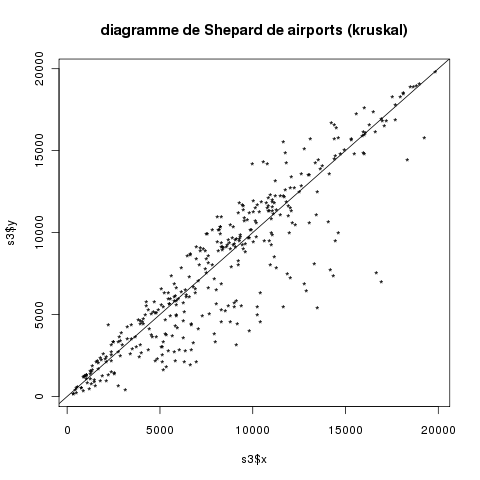
\includegraphics[height = 5cm, width = 5cm]{plots/plot_airports_shepard_kruskal.png}\\ \\
nous pouvons remarquer que les 3 diagrammes observent la même tendance au niveau de la\\disgression pour des valeurs intermédiaires.
Cependant, pour des faibles valeurs, l'utilisation de la méthode de \textit{Sammon} semble plus précise que les 2 autres méthodes.
Donc la méthode de \textit{Sammon} serait plus appropriée pour les petites distances entre aéroports, par exemple les distances
des aéroports à l'intérieur d'un continent.\\ \\
% QUESTION 3
\textbf{Question 3 :}\\
Nous restreignons maintenant les aéroports à l'Europe :\\
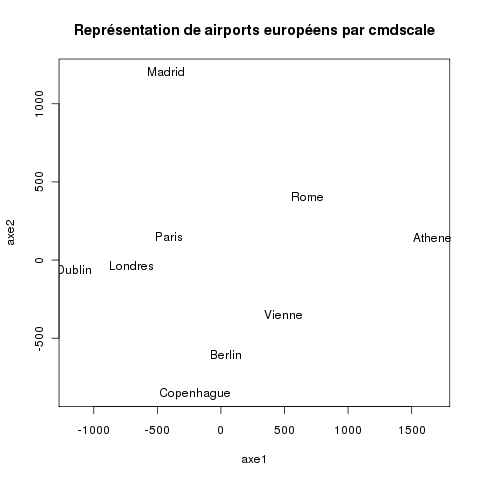
\includegraphics[height = 5cm, width = 5cm]{plots/plot_euro_cmdscale.png}
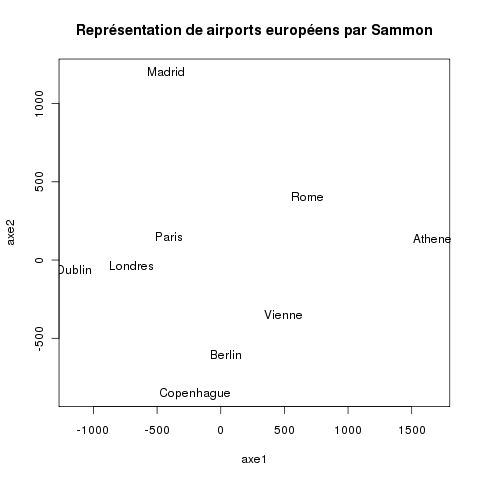
\includegraphics[height = 5cm, width = 5cm]{plots/plot_euro_sammon.png}
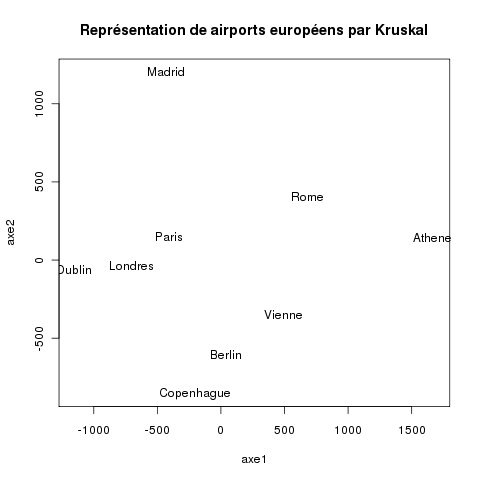
\includegraphics[height = 5cm, width = 5cm]{plots/plot_euro_kruskal.png}\\ \\
Nous pouvons observer que les 3 représentations sont identiques au niveau des distances entre les aéroports européens.
Vu qu'il s'agit de courtes distances où la représentation en 3 dimensions apporte peu de\\modifications des distances,
ces distances dans un espace à 2 dimensions est moins assujettie à des\\variations entre les méthodes utilisées.\\ \\
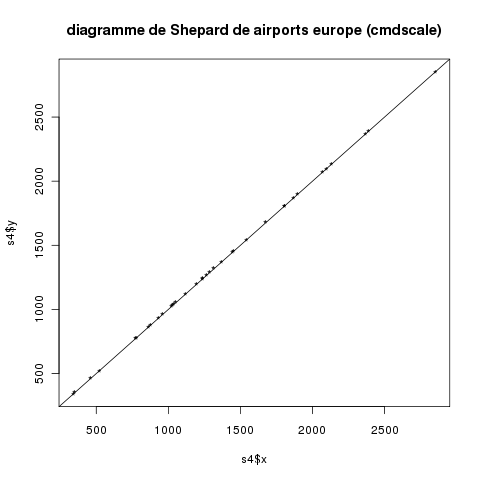
\includegraphics[height = 5cm, width = 5cm]{plots/plot_euro_shepard_cmdscale.png}
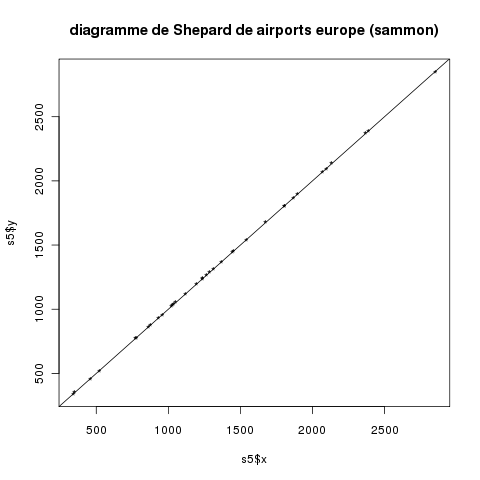
\includegraphics[height = 5cm, width = 5cm]{plots/plot_euro_shepard_sammon.png}
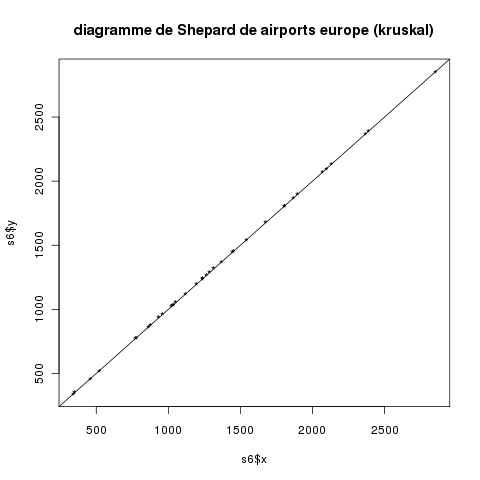
\includegraphics[height = 5cm, width = 5cm]{plots/plot_euro_shepard_kruskal.png}\\ \\
Les diagrammes de \textit{Shepard} pour chacune des méthodes nous montrent que les représentations sont identiques et fiables.
Nous pouvons affirmer que la qualité des résultats dépend donc de la taille de l'échantillon et de la qualité initiale des données.

\section*{Conclusion}
Tout au long de ce tp, nous avons pu voir que chaque méthode de positionnement multidimensionnel (\textit{ACP}, \textit{AFTD},
\textit{Sammon} et \textit{Kruskal}) a ses avantages et ses inconvénients et donc qu'il peut être intéressant
de ne pas se restreindre à l'application d'une seule méthode pour analyser un nuage d'individus selon le type de données initiale.\\
Nous avons pu observer l'utilité du diagramme de \textit{Shepard} pour valider la qualité et la pertinence de l'application d'une méthode
sur un type de données.

\end{document}
